
\begin{IEEEbiography}[{
\includegraphics[width=1in,height=1.25in,clip,keepaspectratio]{fig/kunxie}}]{Kun Xie}
received  PhD
degree in computer application from Hunan University, Changsha, China,
in  2007. She worked as a postdoctoral fellow
in the department of computing in Hong Kong Polytechnic University from
2007.12 to 2010.2. She worked as a visiting researcher in the department
of electrical and computer engineering in state university of New York at
Stony Brook from 2012.9 to 2013.9. Her research interests include wireless network and mobile
computing, network management and control, cloud computing and mobile
cloud, and big data. She has published over 60 papers in major journals and conference proceedings
(including top journals IEEE/ACM TON, IEEE TMC, IEEE TC, IEEE TWC, IEEE TSC, and top conferences INFOCOM, ICDCS, SECON, IWQoS)
\end{IEEEbiography}
\begin{IEEEbiography}[{\includegraphics[width=1in,height=1.25in,clip,keepaspectratio]{fig/taoheng}}]{Heng Tao}
 is now a master student in the department of electrical and computer engineering in state university of New York at
Stony Brook. His research interests include SDN routing and bloom filter.
\end{IEEEbiography}
\begin{IEEEbiography}[{\includegraphics[width=1in,height=1.25in,clip,keepaspectratio]{fig/xinwang}}]{Xin Wang}
 received the Ph.D. degree in electrical and computer engineering from Columbia University, New York, NY.
She is currently an Associate Professor in the Department of Electrical and Computer Engineering of the State University of New York at Stony Brook, Stony Brook, NY. Before joining Stony Brook, she was a Member of Technical Staff in the area of mobile and wireless networking at Bell Labs Research, Lucent Technologies, New Jersey, and an Assistant Professor in the Department of Computer Science and Engineering of the State University of New York at Buffalo, Buffalo, NY. Her research interests include algorithm and protocol design in wireless networks and communications, mobile and distributed computing, as well as networked sensing and detection. She has served in executive committee and technical committee of numerous conferences and funding review panels, and served as the associate editor of IEEE Transactions on Mobile Computing. Dr. Wang achieved the NSF career award in 2005, and ONR challenge award in 2010.
\end{IEEEbiography}




%\begin{IEEEbiography}[{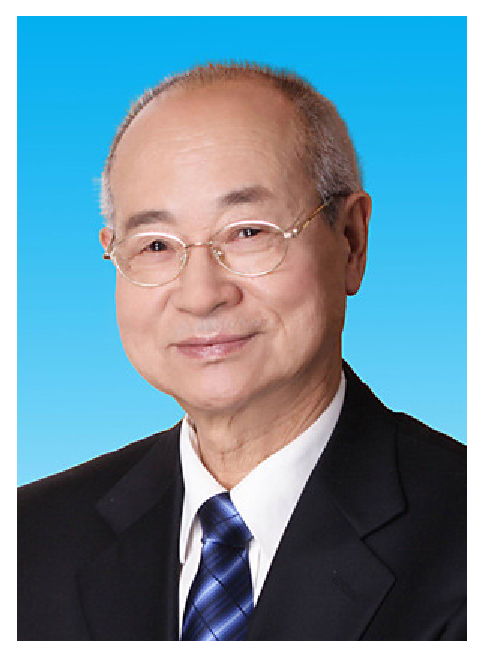
\includegraphics[width=1in,height=1.25in,clip,keepaspectratio]{fig/minyinghua}}]{Yinghua Min} graduated from mathematics department of Jilin university, Changchun, China in 1962, and completed his graduate study in electrical engineering at China Academy of Railway Sciences, Beijing in 1966, although no degree was issued at that time in P.R.China.  He has visited Stanford and other universities in the US for years since 1981.  He is now a professor of Computer science at Institute of Computing Technology, Chinese Academy of Sciences, Beijing, the associate editor-in-chief of 鈥淛ournal of Computer Science and Technology? Honored Chair of technical committee on fault-tolerant computing, China Computer Federation.  He is also a member of the expert committee of the SOC project for the National Natural Science Foundation of China.  He published 230 technical papers, and 4 books, and received the Natural Science award three times from the Chinese Academy of Sciences.  He served as general chairs and program chairs for a number of IEEE symposia and workshops. He is now Co-Chair of the Dragon Star program, a program for US professors to help the People鈥檚 Republic of China (PRC) to improve its graduate education in Computer Science and Engineering. He is a Fellow of IEEE, a member of ACM, and a Golden Core Member of IEEE Computer Society.  His current research interests include electronic testing, dependable computing, and networking.
%\end{IEEEbiography}

%\begin{IEEEbiography}[{
\includegraphics[width=1in,height=1.25in,clip,keepaspectratio]{fig/dafangzhang}}]{Dafang Zhang} received Ph.D. degree in Application Mathematics in Hunan University, Changsha, China, in 1997. He is currently a professor with Hunan University, Changsha, China. His research interests include packet processing, Internet measurement, wireless network and mobile computing, and big data.
%\end{IEEEbiography}

%\begin{IEEEbiography}[{
\includegraphics[width=1in,height=1.25in,clip,keepaspectratio]{fig/dafangzhang}}]{Dafang Zhang} received Ph.D. degree in Application Mathematics in Hunan University, Changsha, China, in 1997. He is currently a professor with Hunan University, Changsha, China. His research interests include packet processing, Internet measurement, wireless network and mobile computing, and big data.
%\end{IEEEbiography}


%\begin{IEEEbiography}[{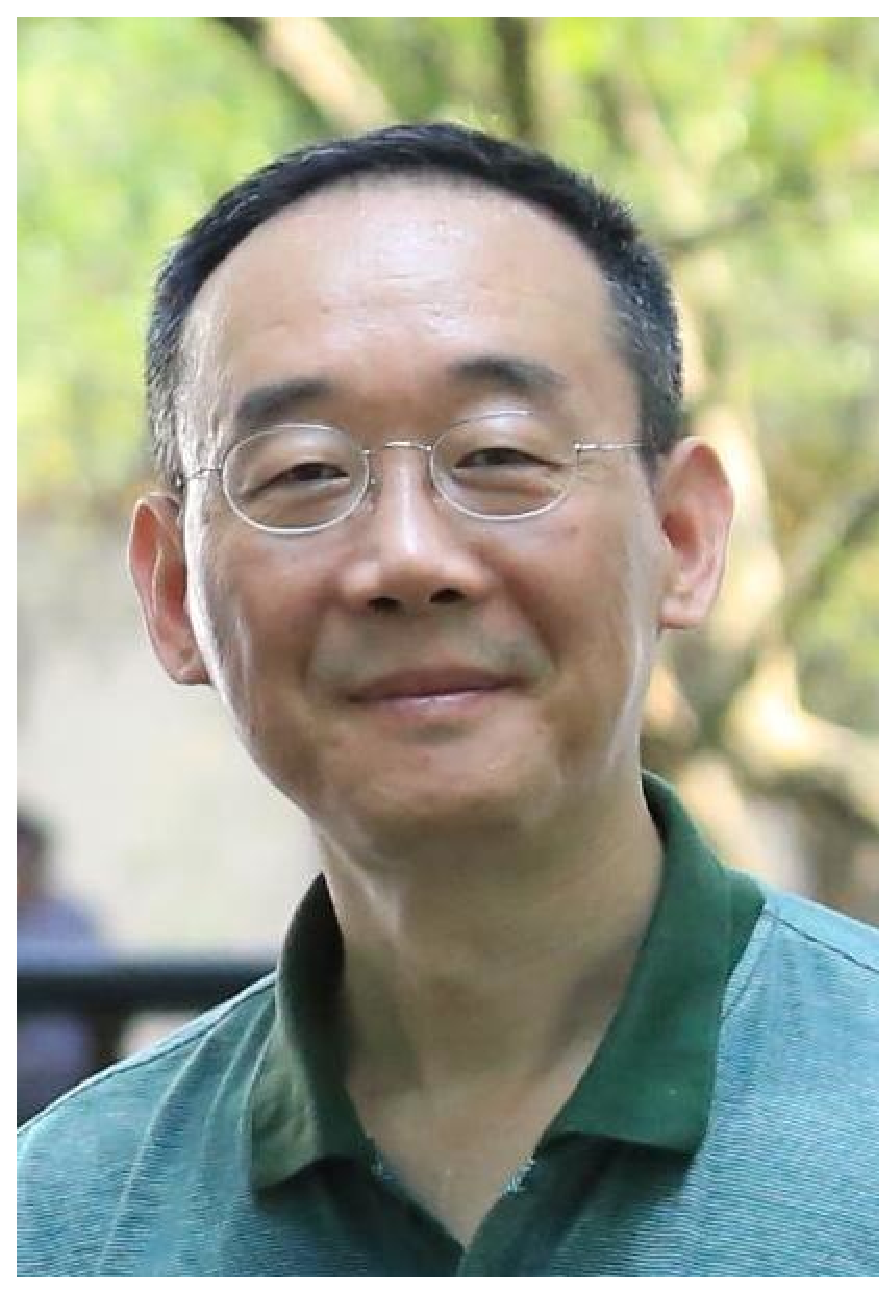
\includegraphics[width=1in,height=1.25in,clip,keepaspectratio]{fig/KeqinLi}}]{Keqin Li} is a SUNY Distinguished Professor of computer science.His current research interests include parallel computing and high-performance computing,
%distributed computing,energy-efficient computing and communication,heterogeneous computing systems,cloud computing,big data computing,CPU-GPU hybrid and cooperative computing,multicore computing,storage and file systems,wireless communication networks,sensor networks,peer-to-peer file sharing systems,mobile computing,service computing,Internet of things and cyber-physical systems.He has published over 400 journal articles, book chapters, and refereed conference papers,and has received several best paper awards.He is currently or has served on the editorial boards of
%{\em IEEE Transactions on Parallel and Distributed Systems},{\em IEEE Transactions on Computers},{\em IEEE Transactions on Cloud Computing},
%{\em Journal of Parallel and Distributed Computing}.He is an IEEE Fellow.
%\end{IEEEbiography}
%\vspace{-30pt}

\begin{IEEEbiography}[{
\includegraphics[width=1in,height=1.25in,clip,keepaspectratio]{fig/gaogangxie}}]{Gaogang Xie}
received his B.S. degree in Physics, M.S. degree and Ph.D. degree in computer science all from Hunan University respectively in 1996, 1999 and 2002. He is currently a Professor and Director of Network Technology Research Center with the Institute of Computing Technology (ICT), Chinese Academy of Sciences (CAS), Beijing, China. His research interests include Internet architecture, packet processing and forwarding, and Internet measurement.
\end{IEEEbiography}

\begin{IEEEbiography}[{
\includegraphics[width=1in,height=1.25in,clip,keepaspectratio]{fig/jigangwen}}]{Jigang Wen}
received PhD degrees in computer application from Hunan University, China, in 2011. He worked as a research assistant in the department of computing in Hong Kong Polytechnic University from 2008 to 2010. He is now a postdoctoral fellow
in Institute of Computing Technology, Chinese Academy of Science, China. His research interests include wireless network and mobile computing, high speed network measurement and management.
\end{IEEEbiography}